\chapter{Testes de Queda}\label{cap:testesdequeda}

\section{Ensaios Experimentais}

Neste capítulo será apresentado a metodologia dos experimentos de teste de queda. Os experimentos foram realizados no Instituto de Tecnologia de Shibaura e na Academia de Defesa Nacional, ambos localizados no Japão, sob supervisionamento dos professores Satoko Abiko e Teppei Tsujita.

O corpo de prova consiste em uma armação retangular com $35mm$ de altura e $100mm$ de largura e comprimento. A armação tem como função proteger e permitir a fixação dos acelerômetros utilizados durante o experimento.
Para garantir uma correta aquisição dos dados e evitar a saturação das acelerações de impacto, dois tipos diferentes de sensores foram utilizados.
No teste com material acolchoado macio, foram aplicados um micro-computador \textit{Intel Edison} e um kit de módulos da \textit{Sparkfun}. O Intel Edison, mostrado na figura \ref{fig:edison}, é equipado com um processador dual-core \textit{Intel Atom} e realiza a comunicação com o módulo 9DoF, equipado com um acelerômetro IMU LSM9DS0, o qual possui uma resolução de $16g$ e uma frequência de $1kHz$.

 \begin{figure}[H]  
        \centering
        \caption{ \textit{Intel Edison} acoplado aos módulos da \textit{Sparkfun}}
        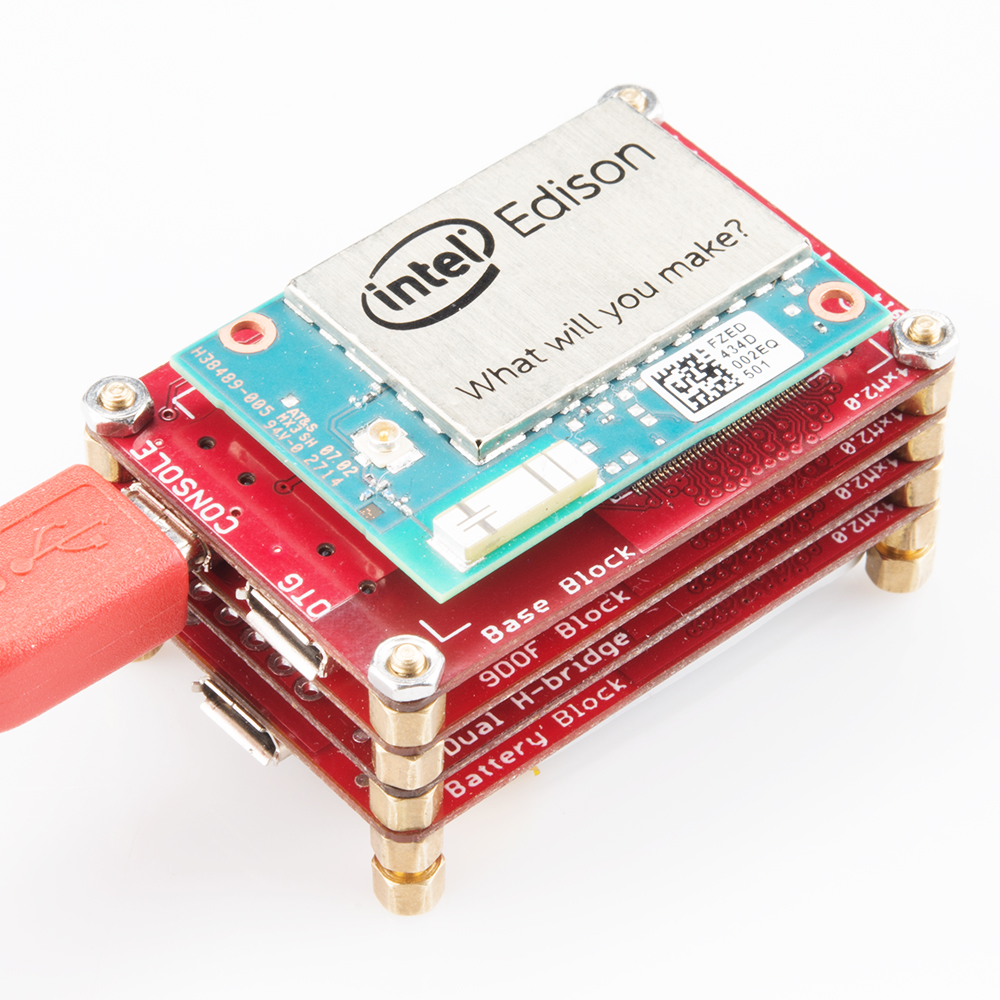
\includegraphics[width=8cm]{./figs/intel_edison.jpg}
        \par\medskip
        Fonte: https://learn.sparkfun.com/tutorials/general-guide-to-sparkfun-blocks-for-intel-edison/all
        \label{fig:edison}
        %https://learn.sparkfun.com/tutorials/general-guide-to-sparkfun-blocks-for-intel-edison/all
\end{figure}

Para o teste com material acolchoado rígido, foi utilizado o acelerômetro da \textit{Microstone} modelo MA3-50AD, mostrado na figura \ref{fig:microstone},  que possui uma resolução de $50g$ a uma frequência de $1kHz$.

 \begin{figure}[H]  
        \centering
        \caption{ Acelerômetro MA3-50AD da \textit{Microstone}.}
        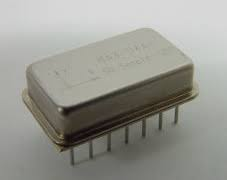
\includegraphics[width=8cm]{./figs/microstone.jpeg}
        \par\medskip
        Fonte: http://microstonecorp.sakura.ne.jp/wp/wp-content/uploads/2018/04/MA3\_R31.pdf
        \label{fig:microstone}
\end{figure}

Na face superior, uma chapa de metal foi fixada de modo a possibilitar a suspensão do corpo de teste por um eletroímã. já na face inferior, foram fixados os materiais acolchoados que seriam submetidos para análise. Adicionalmente, 6 pequenas esferas cinza foram coladas ao redor do corpo de teste. Por meio de 6 câmeras de captura de movimento, o software \textit{Optitrack:Motive} monitora a posição das esferas cinzas. Desse modo, tanto a aceleração como a posição do dispositivo são obtidos durante o ensaio experimental.

O dispositivos descritos são mostrados nas figuras \ref{fig:CorpoDeProva2} e \ref{fig:SoftCorpo} a seguir:

 \begin{figure}[H]  
        \centering
        \caption{Corpo de prova com material acolchoado rígido contendo os marcadores esféricos cinzas e, no centro da estrutura, o acelerômetro MA3-50AD da \textit{Microstone}.}
        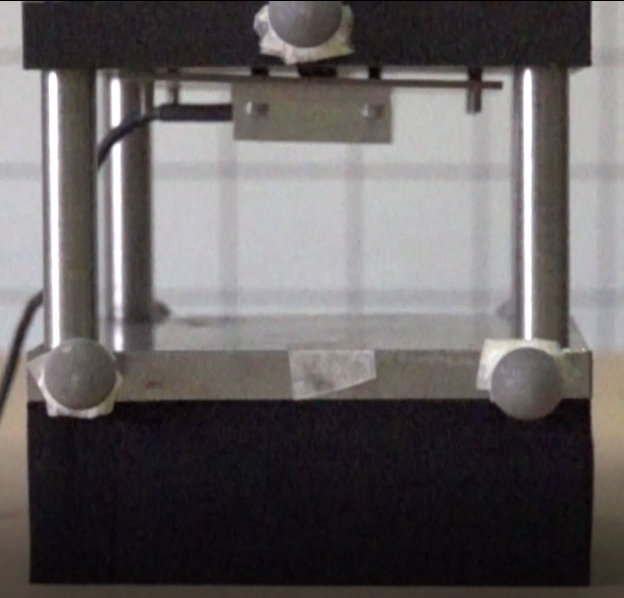
\includegraphics[width=8cm]{./figs/CorpoDeProva.PNG}
        \par\medskip
        Fonte: Própria autoria.
        \label{fig:CorpoDeProva2}
\end{figure}

 \begin{figure}[H]  
        \centering
        \caption{Corpo de prova com material acolchoado macio, pode-se observar os marcadores esféricos cinzas fixados na estrutura, a chapa metálica no topo do dispositivo e no centro, o conjunto \textit{Intel Edison} e os módulos para aquisição de dados.}
        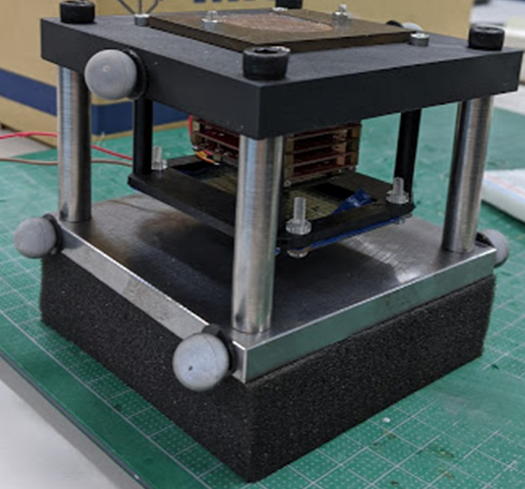
\includegraphics[width=8cm]{./figs/soft_drop_test.PNG}
        \par\medskip
        Fonte: Própria autoria.
        \label{fig:SoftCorpo}
\end{figure}

Duas câmeras foram utilizadas para a captura visual do experimento. A primeira, a câmera \textit{Sony HDR-CX900} foi utilizada para a filmagem e gravação do áudio de uma visão ampla do experimento. A segunda, \textit{Sony RX100M5}, é uma câmera \textit{High Frame Rate} (HFR) utilizada para produzir vídeos em câmera lenta, sendo capaz de registaté 960 quadros por segundo \cite{sonyHFR}. Ela foi utilizada para capturar a deformação do material acolchoado durante o impacto ao solo.

Para cada material acolchoado, foram realizados testes de queda utilizando alturas de $5cm$ e $8cm$. O dispositivo suspendido foi por um eletroímã, alimentado por uma fonte de tensão DC. Um goniômetro digital foi utilizado para garantir que o solo e a face inferior do corpo de prova estivessem paralelas. Para reduzir o impacto e proteger os dispositivos eletrônicos utilizados durante o teste, o chão foi forrado com o material acolchoado rígido.

A figura \ref{fig:environment} mostra o ambiente de experimentos:

 \begin{figure}[H]  
        \centering
        \caption{\textit{Setup} utilizado para os testes de queda.}
        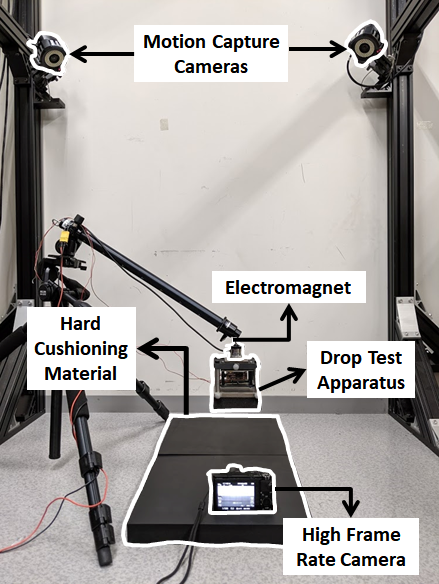
\includegraphics[width=8cm]{./figs/environment.PNG}
        \par\medskip
        Fonte: Própria autoria.
        \label{fig:environment}
\end{figure}

Para cada experimento, o dispositivo é suspenso pelo eletroímã e a altura é medida e ajustada com uma fita-métrica. O goniômetro é utilizado para se certificar que o solo e o corpo de testes estejam paralelos entre si.
Uma vez calibrados, as câmeras, o software de captura de movimento e os sensores são ativados, iniciando a coleta de dados. Após essa etapa, a alimentação do eletroímã é cortada, levando o corpo de prova a uma queda-livre até o impacto ao solo. No final do teste, os dados são reunidos para uma posterior análise.

\section{Simulação do Teste de Queda}

Para a simulação do teste de queda, um programa de \textit{Matlab} foi desenvolvido no ambiente \textit{Simulink}, com o pacote de ferramentas \textit{Simscape Multibody Toolbox}.

O \textit{Simscape Multibody Toolbox} possibilita a simulação 3D de sistemas mecânicos de multicorpos. A construção de modelos é simplificada por meio de diagramas de bloco, os quais podem representar corpos, juntas, forças ou sensores. Outra vantagem é que o \textit{Simscape Multibody Toolbox} formula e resolve as equações de movimento para todo o sistema \cite{simscape}.

No teste de queda, conforme mencionado na seção anterior, uma armação de metal é utilizada para proteger os sensores e fixar o material acolchoado. Um modelo CAD desta armação foi construída em \textit{Solidworks}, mostrado na fig. \ref{fig:corpodeprovacad}, com o objetivo de obter suas características físicas, como matriz de inércia, centro de massa.

 \begin{figure}[H] 
        \centering
        \caption{Armação de metal construído em \textit{Solidworks}.}
        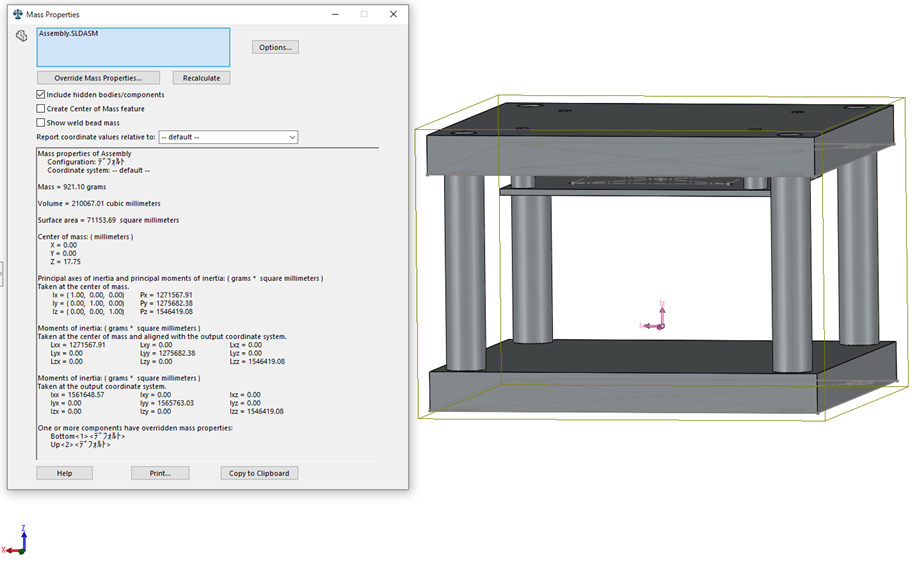
\includegraphics[width=8cm]{./figs/corpodeprova_cad.png}
        \par\medskip
        Fonte: Própria autoria.
        \label{fig:corpodeprovacad}
        %https://learn.sparkfun.com/tutorials/general-guide-to-sparkfun-blocks-for-intel-edison/all
\end{figure}

Essas características físicas são configuradas no modelo simplificado da armação de metal. Nele, sua modelagem é feitos através de um prisma retangular rígido com as mesmas propriedades da peça construída em \textit{Solidworks}. Embora o \textit{Simscape Multibody Toolbox} permita a importação da peça CAD no \textit{Simulink}, seu uso causou instabilidade nas simulações. Desse modo, optou-se em utilizar o modelo simplificado.
O material acolchoado é representado da mesma forma, por um prima retangular, anexado na face inferior da armação de metal, mostrados na fig. \ref{fig:corpodeprovasimulink}, 

 \begin{figure}[H] 
        \centering
        \caption{Ambiente de teste de queda do Simulink, com o corpo de prova. A armação de metal em azul e material acolchoado em cinza}
        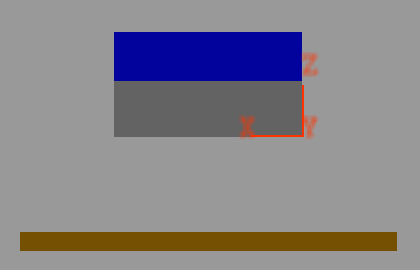
\includegraphics[width=8cm]{./figs/corpodeprova_simulink.png}
        \par\medskip
        Fonte: Própria autoria.
        \label{fig:corpodeprovasimulink}
        %https://learn.sparkfun.com/tutorials/general-guide-to-sparkfun-blocks-for-intel-edison/all
\end{figure}

Vale destacar que no ambiente do \textit{Simulink}, o material acolchoado é tratado como rígido e \textit{Simscape Multibody Toolbox} não calcula as deformações do material, mas a dinâmica do corpo de teste influenciada pela força e torque gerado no impacto com o solo. 
Como será explicado a seguir deste capítulo, uma função a parte será responsável pelo cálculo da deformações do material, e pela força e torque resultantes do impacto ao solo.

Uma das dificuldades da simulação do teste de impacto está na modelagem da força de reação do solo.
Com o material teórico apresentado no capítulo \ref{cap:elementosfinitos}, serão apresentados dois modelos elaborados para essa finalidade. No primeiro modelo, considera-se a força de reação do solo como sendo proporcional ao deslocamento e velocidade dos nós que atravessam o chão. No segundo modelo, considera-se o deslocamento dos nós dentro do solo. 

\subsection{Modelo da Força de Reação do Solo}

Neste modelo, representado na fig. \ref{fig:reactionforcemodel}, o material acolchoado é discretizado por elementos finitos, conforme detalhado no capítulo \ref{cap:elementosfinitos}. Os nós que compõem essa malha são identificados em um de dois grupos. No primeiro estão os nós chamados de fixos, $u_{fix}$, estes nós estão fixados à armação de metal, e assim não possuem deslocamento em relação ao sistema de coordenadas local. Os restantes, chamados de nós livres, $u_{free}$, podem sofrer deformações. 
Para cada nó $j$ da malha, sua posição é dada por:

\begin{equation} \label{eq:position}
    p_{j} = 
    \begin{bmatrix}
        p_{x,j}
        \\
        p_{y,j}
        \\
        p_{z,j}
    \end{bmatrix}
\end{equation}
onde $p_{x,j}, (p_{y,j}, p_{z,j})$ são, respectivamente, as componentes de $p_{j}$ nos eixos $x$, $y$ e $z$.

 \begin{figure}[H] 
        \centering
        \caption{Modelo da Força de Reação do Solo.}
        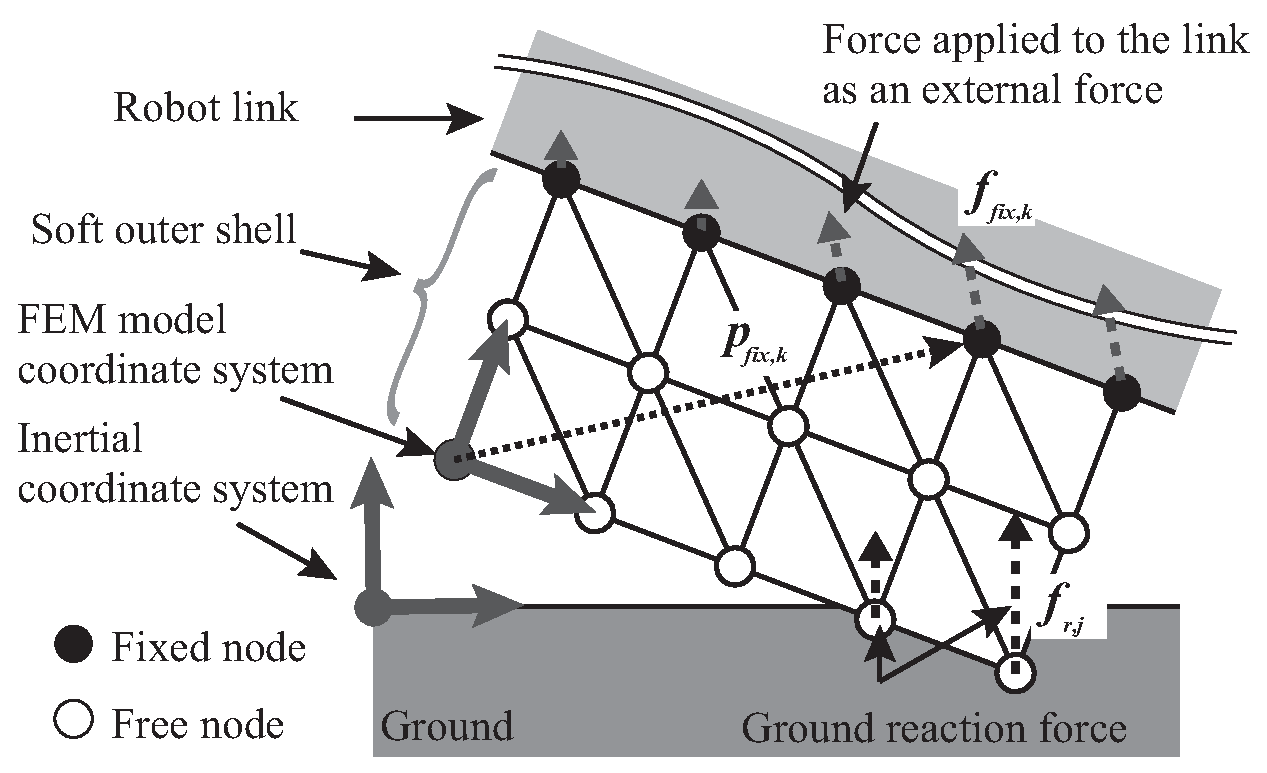
\includegraphics[width=8cm]{./figs/fig2_FEM-MBD_model.eps}
        \par\medskip
        Fonte: 
        \label{fig:reactionforcemodel}
        %https://learn.sparkfun.com/tutorials/general-guide-to-sparkfun-blocks-for-intel-edison/all
\end{figure}

Uma vez identificados, o conjunto $U$ de nós que compõem a malha são reordenados da seguinte maneira:

\begin{equation} \label{eq:fixfreenodes}
    U = 
    \begin{bmatrix}
        u_{free}
        \\
        u_{fix}
    \end{bmatrix}
\end{equation}
onde $u_{free}$ é o conjunto de nós livres e $u_{fix}$ o conjunto de nós fixos.

A força de reação do solo, para o nó $j$ da malha, é definido como \cite{nenchev2018humanoid}:

\begin{equation} \label{eq:floor_force}
        f_{r,j} &= \begin{cases}
    \begin{bmatrix}
        0
        \\
        0
        \\
        -K_{ground}(p_{z,j} - H_{ground}) - D_{ground}\dot{p}_{z,j}
    \end{bmatrix} &\textrm{, se $(p_{z,j} - H_{ground})  < 0$} \\
    
    \begin{bmatrix}
        0
        \\
        0
        \\
        0 
        \end{bmatrix} & \textrm{, caso contrário} \\ 
        \end{cases}
\end{equation}
onde $K_{ground}$ e $K_{ground}$ são, respectivamente, a constante elástica e amortecimento do solo. São parâmetros escolhidos manualmente para a simulação, e possuem os seguintes valores: $K_{ground} = 600$ e $K_{ground} = 0.6$. $(p_{z,j}$ e $\dot{p}_{rz,j}$ são, respectivamente, as componentes no eixo-z da posição e velocidade do nó $j$, escritas no sistema de coordenada global. $H_{ground}$ representa o nível do solo.

Uma vez definido a força $f_{r}$, pode-se escrever a eq. \ref{eq:dynamic} para o conjunto $U$ de nós da malha:

\begin{equation} \label{eq:dynamic}
\pmb{M}\ddot{\pmb{u}} + \pmb{D}\dot{\pmb{u}} + \pmb{K}\pmb{u} = \pmb{f} 
\end{equation}
reordenando os nós conforme \ref{eq:fixfreenodes} e calculando as matrizes $\pmb{M}$, $\pmb{D}$ e $\pmb{K}$, \ref{eq:dynamic} se torna:

\begin{equation} \label{eq:block_dynamic}
     \begin{bmatrix}
            \pmb{M}_0 \quad \pmb{M}_1 \\
            \pmb{M}_2 \quad \pmb{M}_3
    \end{bmatrix}
     \begin{bmatrix}
       \ddot{\pmb{u}}_{free} \\
       \ddot{\pmb{u}}_{fix} 
    \end{bmatrix}    
    + \begin{bmatrix}
            \pmb{D}_0 \quad \pmb{D}_1 \\
            \pmb{D}_2 \quad \pmb{D}_3
         \end{bmatrix}
         \begin{bmatrix}
            \dot{\pmb{u}}_{free} \\
            \dot{\pmb{u}}_{fix} 
         \end{bmatrix}
    + \begin{bmatrix}
            \pmb{K}_0 \quad \pmb{K}_1 \\
            \pmb{K}_2 \quad \pmb{K}_3
         \end{bmatrix}
         \begin{bmatrix}
            \pmb{u}_{free} \\
            \pmb{u}_{fix} 
         \end{bmatrix} =
         \begin{bmatrix}
            \pmb{f}_{free} \\
            \pmb{f}_{fix} 
    \end{bmatrix}
\end{equation}
onde, $u_{fix}$, $\dot{u}_{fix}$ e $\ddot{u}_{fix}$
são, respectivamente, o deslocamento dos nós fixo e suas primeira e segunda derivadas temporais. Como esses nós estão fixos na estrutura, seus valores são nulos. $f_{free}$ é calculado a partir de \ref{eq:floor_force}.
$u_{free}$, $\dot{u}_{free}$, $\ddot{u}_{free}$ e $f_{fix}$ são as incónitas a se determinar.
Da eq. \ref{eq:block_dynamic}, pode-se escrever:

\begin{equation} \label{eq:ufree_calc}
    \pmb{u}_{free} = \pmb{K}_0^{-1}(\pmb{f}_{free} - \pmb{D}_0 \dot{\pmb{u}}_{free} -\pmb{M}_0\ddot{\pmb{u}}_{free})     
\end{equation}
\begin{equation} \label{eq:force_fix_cal}
     \pmb{f}_{fix} = \pmb{K}_2 \pmb{u}_{free} + \pmb{D}_2 \dot{\pmb{u}}_{free} + \pmb{M}_2 \ddot{\pmb{u}}_{free}       
\end{equation}
$u_{free}$, $\dot{u}_{free}$, $\ddot{u}_{free}$ são obtidos resolvendo \ref{eq:ufree_calc} com o método de integração númerica de Newmark, apresentado no capítulo \ref{cap:elementosfinitos}. Uma vez obtidos esses valores, $f_{fix}$ é calculado com a eq. \ref{eq:force_fix_cal}.

Calcula-se o versor de força externa $\mathcal{F}_i$, em relação ao Sistema de Coordenadas Local:

\begin{equation} \label{eq:externalforcetorque}
\pmb{\mathcal{F}}_i
=  \begin{bmatrix}
        \sum_{k=1}^{N_{fix}} \pmb{f}_{fix,k} \\[1em]
        \ \sum_{k=1}^{N_{fix}} \pmb{p}_{fix,k}\times \pmb{f}_{fix,k} \ 
     \end{bmatrix}
\end{equation}
onde $f_{fix}$ é a força aplicada no nó fixo $k$ e $p_{fix}$ é a posição do nó fixo $k$, em relação ao Sistema de Coordenada Local.

Finalmente, os valores de deslocamentos são somados à posição inicial no instante $t$ de cada nó. E essa nova posição é utilizada como posição inicial no seguinte ciclo, $t+1$.

\begin{equation} \label{eq:newposition}
    p^{t+1}_{j} = p^{t}_{j} + u_{j}
\end{equation}


\subsection{Modelo do Deslocamento no Solo}

Neste modelo, representado na fig. \ref{fig:displacementmodel}, o material acolchoado é discretizado por elementos finitos, conforme detalhado no  
capítulo \ref{cap:elementosfinitos}. Os nós que compõem essa malha são identificados em um de dois grupos. No primeiro estão os nós de contato, $U_{con}$. Estes são nós que estão em contato com o solo ou com a armação de metal. Os demais nós, assim como no modelo anterior, são chamados de nós livres, $U_{free}$.
Para cada nó $j$ da malha, sua posição é dada por:

\begin{equation} \label{eq:position}
    p_{j} = 
    \begin{bmatrix}
        p_{x,j}
        \\
        p_{y,j}
        \\
        p_{z,j}
    \end{bmatrix}
\end{equation}
onde $p_{x,j}, (p_{y,j}, p_{z,j})$ são, respectivamente, as componentes de $p_{j}$ nos eixos $x$, $y$ e $z$.

 \begin{figure}[H] 
        \centering
        \caption{Modelo do Deslocamento no Solo.}
        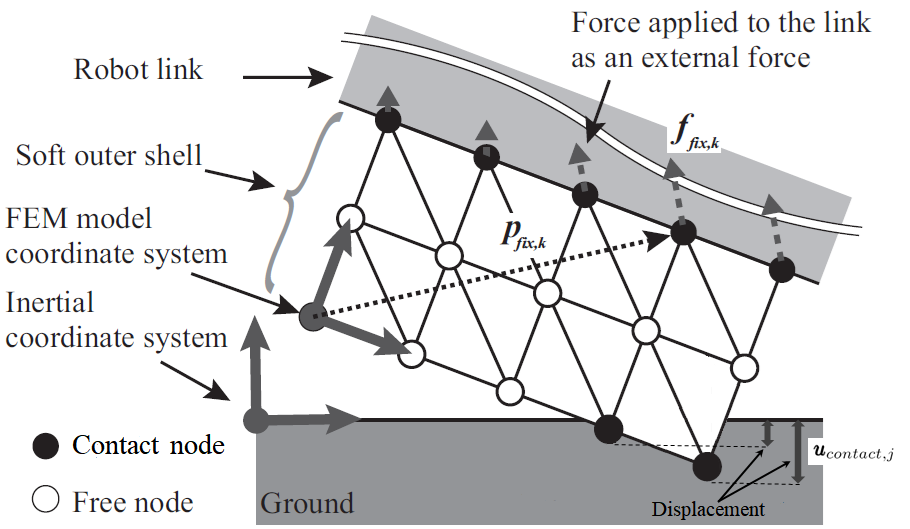
\includegraphics[width=8cm]{./figs/ForcedDisplacementFinal.png}
        \par\medskip
        Fonte: 
        \label{fig:displacementmodel}
        %https://learn.sparkfun.com/tutorials/general-guide-to-sparkfun-blocks-for-intel-edison/all
\end{figure}

Uma vez identificados, o conjunto $U$ de nós que compõem a malha são reordenados da seguinte maneira:

\begin{equation} \label{eq:fixfreenodes}
    U = 
    \begin{bmatrix}
        u_{free}
        \\
        u_{con}
    \end{bmatrix}
\end{equation}
onde $u_{free}$ é o conjunto de nós livres e $u_{con}$ o conjunto de nós de contato.

Ao contrário do modelo anterior, para resolver a eq. \ref{eq:dynamic}, não será calculada a força de reação do solo para cada nó. Ao invés disso, será utilizado o deslocamento dos nós abaixo do solo. Para o nó de contato $j$, seu deslocamento, em relação ao sistema de coordenadas global, é dado por:

\begin{equation} \label{eq:floordisp}
        u^{g}_{con,j} &= \begin{cases}
    \begin{bmatrix}
        0
        \\
        0
        \\
         H_{ground} - {p}_{z,j})
    \end{bmatrix} &\textrm{, se $H_{ground} - {p}_{z,j}) < 0$} \\
    
    \begin{bmatrix}
        0
        \\
        0
        \\
        0 
        \end{bmatrix} & \textrm{, caso contrário} \\ 
        \end{cases}
\end{equation}
onde, $H_{ground}$ e ${p}_{z,j}$ são, respectivamente, o nível do solo e a componente do eixo-$z$ da posição do nó $j$, ambos em relação ao sistema de coordenadas global.

Para expressar o deslocamento em termos do sistema de coordenadas local, uma transformação de coordenadas é aplicado:

\begin{equation} \label{eq:localglobaldisp}
    u_{con, j} = \pmb{R}u^{g}_{con, j} 
\end{equation}

onde $\pmb{R}$ é a matriz de rotação $R$ do sistema de coordenadas global para o sistema de coordenadas local. $u_{con, j}$ é o deslocamento do nó de contato $j$, no sistema de coordenadas local.

Pode-se calcular $\dot{u}_{con}$ e $\ddot{u}_{con}$ da seguinte forma:

\begin{equation}\label{eq:velocdisp}
    \dot{u}_{con} = \frac{{u}_{con}}{\Delta t}
\end{equation}

\begin{equation} \label{eq:accdisp}
        \ddot{u}_{con} = \frac{{\dot{u}}_{con}}{\Delta t}
\end{equation}
onde $\Delta t$ é o intervalo de tempo da simulação.

Reordenando os nós conforme \ref{eq:fixfreenodes} e calculando as matrized $\pmb{M}$, $\pmb{D}$ e $\pmb{K}$, a equação \ref{eq:dynamic} por ser escrita como:

\begin{equation} \label{eq:blockdisp}
 \begin{bmatrix}
        \pmb{M}_0 \quad \pmb{M}_1 \\
        \pmb{M}_2 \quad \pmb{M}_3
\end{bmatrix}
 \begin{bmatrix}
   \ddot{\pmb{u}}_{free} \\
   \ddot{\pmb{u}}_{con} 
\end{bmatrix}    
+ \begin{bmatrix}
        \pmb{D}_0 \quad \pmb{D}_1 \\
        \pmb{D}_2 \quad \pmb{D}_3
     \end{bmatrix}
     \begin{bmatrix}
        \dot{\pmb{u}}_{free} \\
        \dot{\pmb{u}}_{con} 
     \end{bmatrix}
+ \begin{bmatrix}
        \pmb{K}_0 \quad \pmb{K}_1 \\
        \pmb{K}_2 \quad \pmb{K}_3
     \end{bmatrix}
     \begin{bmatrix}
        \pmb{u}_{free} \\
        \pmb{u}_{con} 
     \end{bmatrix} =
     \begin{bmatrix}
        \pmb{f}_{free} \\
        \pmb{f}_{con} 
\end{bmatrix}
\end{equation}
onde $\ddot{u}_{con}$, $\dot{u}_{con}$ e $u_{con}$ são encontrados através das equações \ref{eq:floordisp}, \ref{eq:localglobaldisp}, \ref{eq:velocdisp} e \ref{eq:accdisp}. Além disso $f_{free}$ é um vetor nulo, pois os nós livres não estão sujeitos à força de reação do solo.
Assim $\ddot{u}_{free}$, $\dot{u}_{free}$, $u_{free}$ e $f_{con}$ são as incógnitas a serem calculadas.

Da eq. \ref{eq:blockdisp} pode-se escrever as seguintes equações:

\begin{equation} \label{eq:udispcalc}
    \pmb{M}_0\ddot{\pmb{u}}_{free} +  \pmb{C}_0\dot{\pmb{u}}_{free} +  \pmb{K}_0\pmb{u}_{free} = \pmb{f}_{free} - (\pmb{M}_1\ddot{\pmb{u}}_{con} +  \pmb{C}_1\dot{\pmb{u}}_{con} +  \pmb{K}_1\pmb{u}_{con}) 
\end{equation}

\begin{equation} \label{fdispcalc}
    \pmb{f}_{con} =  \pmb{M}_2\ddot{\pmb{u}}_{free} +  
    \pmb{C}_2\dot{\pmb{u}}_{free} +  \pmb{K}_2\pmb{u}_{free} + 
    \pmb{M}_3\ddot{\pmb{u}}_{con} +  \pmb{C}_3\dot{\pmb{u}}_{con} + \pmb{K}_3\pmb{u}_{con}
\end{equation}
$\ddot{u}_{free}$, $\dot{u}_{free}$ e $u_{free}$ são calculados resolvendo a eq. \ref{eq:udispcalc} através do método de integração numérica apresentado no capítulo \ref{cap:elementosfinitos}. Com estes resultados, encontra-se $f_{con}$ resolvendo a eq. \ref{eq:floordisp}.
 
 A seguir, calcula-se o versor de força externa $\mathcal{F}_i$, em relação ao Sistema de Coordenadas Local:

\begin{equation} \label{eq:externalforcetorque}
\pmb{\mathcal{F}}_i
=  \begin{bmatrix}
        \sum_{k=1}^{N_{con}} \pmb{f}_{con,k} \\[1em]
        \ \sum_{k=1}^{N_{con}} \pmb{p}_{con,k}\times \pmb{f}_{con,k} \ 
     \end{bmatrix}
\end{equation}
onde $f_{con}$ é a força aplicada no nó fixo $k$ e $p_{con}$ é a posição do nó fixo $k$, em relação ao sistema de coordenada local.

Finalmente, os valores de deslocamentos são somados à posição inicial no instante $t$ de cada nó. E essa nova posição é utilizada como posição inicial no seguinte ciclo, $t+1$.

\begin{equation} \label{eq:newposition}
    p^{t+1}_{j} = p^{t}_{j} + u_{j}
\end{equation}

\section{Implementação no Matlab}

